%% Example data sheet
%% Feel free to modify and use this file for any purpose, under
%% either the LaTeX Project Public License or under public domain.

% Options here are passed to the article class.
% Most common options: 10pt, 11pt, 12pt
\documentclass[10pt]{datasheet}

% Input encoding and typographical rules for English language
\usepackage[utf8]{inputenc}
\usepackage[english]{babel}
\usepackage[english]{isodate}

% tikz is used to draw images in this example, but you can
% also use \includegraphics{}.
\usepackage{tikz}
\usepackage{pgfplots}
\usepackage{circuitikz}
\usetikzlibrary{calc}

% These define global texts that are used in headers and titles.
\title{ETL Tamale Module Design}
\author{ETL Module design team}
\date{June 2022}
\revision{Revision 1}
\companylogo{\Huge CMS}

\begin{document}
\maketitle

\section{Features}

\begin{itemize}
\item{TBD}
\item{TBD}
\item{TBD}
\end{itemize}

\section{General Description}
TBD TBD

% Switch to next column
\vfill\break

\begin{figure}[h]
    \begin{circuitikz}[european]
        \node[op amp] (amp1) {};
        \node[op amp, below = 0.5cm, xscale = -1] (amp2) {};
        \draw (amp1.out) |- (amp2.-);
        \draw (amp2.-) ++(0, 0.3cm) node[circ]{} to +(2,0) node[above left]{5};
        \draw (amp2.out) to (amp1.+);
        \draw (amp1.+) ++(0, -0.3cm) node[circ]{} to +(-2,0) node[above right]{2};
        \draw (amp1.-) to +(-2,0) node[above right]{1};
        \draw (amp2.+) to +(2,0) node[above left]{4};
        \draw (amp1.out) +(0,0.5cm) node (Vdd) {$\mathrm{V_{DD}}$};
        \draw (Vdd.east) to +(1.5,0) node [above left]{6};
        \draw (amp2.out) +(0,-0.5cm) node (Vss) {$\mathrm{V_{SS}}$};
        \draw (Vss.west) to +(-1.6,0) node [above right]{3};
        \draw ($(amp1.north west) + (-0.5,0.5)$) rectangle ($(amp2.south west) + (0.5,-0.5)$);
    \end{circuitikz}
    \caption{Pinout and internal circuit}
\end{figure}

\begin{figure}[h]
    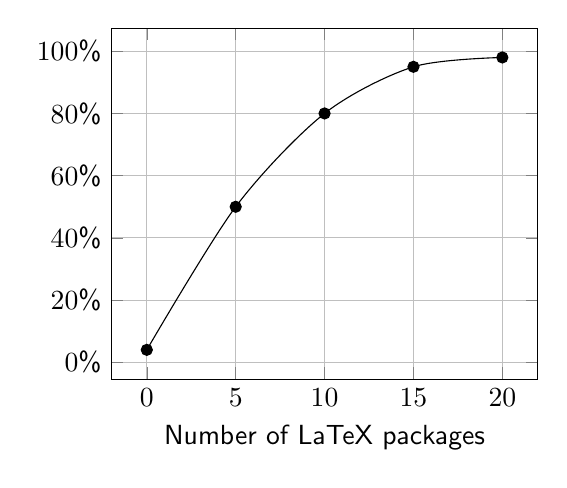
\begin{tikzpicture}
        \sffamily
        \begin{axis}[
            width=7cm,
            xlabel={Number of LaTeX packages},
            ytick distance=20,
            yticklabel={\pgfmathprintnumber{\tick}\%},
            xmajorgrids, ymajorgrids]
        \addplot[smooth,mark=*] plot coordinates {
            (0,4)
            (5,50)
            (10,80)
            (15,95)
            (20,98)
        };
        \end{axis}
    \end{tikzpicture}
    \caption{Typical data sheet production efficiency}
\end{figure}

% For wide tables, a single column layout is better. It can be switched
% page-by-page.
\onecolumn

\section{Overview of Design}

\section{ETROC \& LGAD Subassembly}

\section{Module PCB}

\section{Baseplate}

\section{Ahesive Films}

\end{document}


